\documentclass[conference]{IEEEtran}
\IEEEoverridecommandlockouts
% The preceding line is only needed to identify funding in the first footnote. If that is unneeded, please comment it out.
\usepackage{cite}
\usepackage{amsmath,amssymb,amsfonts}
\usepackage{algorithmic}
\usepackage{graphicx}
\usepackage{textcomp}
\usepackage{xcolor}
\def\BibTeX{{\rm B\kern-.05em{\sc i\kern-.025em b}\kern-.08em
    T\kern-.1667em\lower.7ex\hbox{E}\kern-.125emX}}
\begin{document}

\title{Mission Planning Tool for Space Debris Detection and Tracking with the MeerKAT Radar\\
\thanks{*This work was supported by funding from the South African Radio Astronomy Observatory}
}

\author{\IEEEauthorblockN{Ashiv Dhondea, MR Inggs}
\IEEEauthorblockA{\textit{Radar Remote Sensing Group} \\
\textit{University of Cape Town}\\
Rondebosch, South Africa\\
ashivdhondea5@gmail.com, mikings@gmail.com}
%\and
%\IEEEauthorblockN{MR Inggs}
%\IEEEauthorblockA{\textit{Radar Remote Sensing Group} \\
%\textit{University of Cape Town}\\
%Cape Town, South Africa \\
%mikings@gmail.com}
}

\maketitle

\begin{abstract}
Sustained human activity in Space has had the unfortunate consequence of creating space debris which accumulate in orbit. The rubble cloud which arose in the LEO regime poses a significant collision risk for spacecraft. Space surveillance is crucial to predict and prevent potential collisions in orbit. Surveillance and tracking are done with radar and telescope systems. A bistatic radar system featuring the MeerKAT radio telescope in South Africa as its receiver network has been proposed to perform space debris detection and tracking. This paper describes the Mission Planning Tool developed to perform sensor scheduling and predicting the performance of the proposed MeerKAT radar in terms of orbit determination accuracy. Numerical simulation results are shown to illustrate the operation of the proposed MeerKAT radar system for space target observation.
\end{abstract}

\begin{IEEEkeywords}
space debris, bistatic radar, orbit determination, radio telescope, mission planning
\end{IEEEkeywords}

\section{INTRODUCTION}
Space debris pose an extremely concerning collision threat to Man's valuable spacecraft in orbit: not only can a piece of space rubble collide with a spacecraft at a very high relative velocity and put it out of commission, it can also collide with another piece of junk, thereby creating a multitude of smaller particles which eventually spread out in orbit and increase the chances of collision with an important space asset.

According to NASA's Orbital Debris Program Office (ODPO) in \cite{odpo}, there are more than 21000 space debris objects which exceed $10~\mathrm{cm}$ in size in Earth orbit. The clutter in the LEO regime will grow exponentially over time if no countermeasures are taken. The rising uncertainty in the safety of the space environment in the early 2000s led to the emergence of the concept of Space Situational Awareness (SSA) \cite{mehrholz2002detecting}. SSA is defined as the thorough knowledge of the space environment, which incorporates the ability to track and predict the location of space objects (RSOs) at any time \cite{spsiaw}. The European Space Agency in \cite{esaklinkrad,krag2010european} identified the first aspect of SSA to be SST: Space Surveillance and Tracking of resident space objects. 

In the light of this, the University of Cape Town's Radar Remote Sensing Group is performing a feasibility and design study for a potential bistatic radar featuring the MeerKAT radio telescope as radar receiver (Rx) \cite{doreenphd}. The MeerKAT array consists of 64 dishes and is currently being built by the South African Radio Astronomy Observatory, in the Northern Cape Province of South Africa. The proposed transmitter (Tx) is proposed to be located the Denel Dynamics' Overberg test range in Arniston, Bredasdorp (Western Cape, South Africa). Figure \ref{fig:map} is a map indicating the location of the radar Rx and Tx. The bistatic baseline, indicated by the red line in Figure \ref{fig:map}, is $443.787~\mathrm{km}$ long. At the current initial stage of the MeerKAT radar design, the goal of the proposed system is to improve the monitoring from the Southern hemisphere of small space debris populating the Low Earth Orbit regime.

\begin{figure}[t]
	\centering
	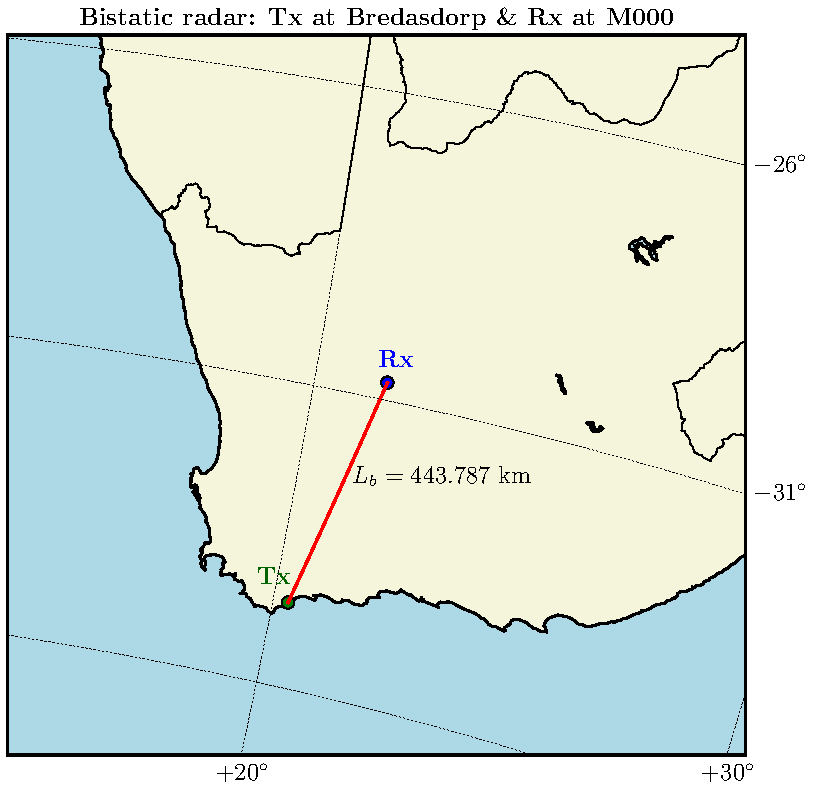
\includegraphics[scale=0.48]{bisradvisual.pdf}
	\caption{Map showing the location of the Tx in Bredasdorp at $34.6\mathrm{^\circ}\text{S}$ and $20.3\mathrm{^\circ}\text{E}$ and Rx at Carnarvon at $30.7\mathrm{^\circ}\text{S}$ and $21.4\mathrm{^\circ}\text{E}$.} 
	\label{fig:map}
\end{figure}
%\todo[inline]{The standard is to put an overview of the rest of the paper here, referring to each section}
This paper describes the Mission Planning Tool (MPT) developed to perform sensor scheduling and predicting the performance of the proposed MeerKAT radar in terms of orbit determination accuracy \cite{ashivmsc}. Numerical simulation results are shown to illustrate the operation of the proposed MeerKAT radar system for space target observation. Targets considered in the study \cite{ashivmsc} were known satellites and space debris which originated from Fengyun-1C, Kosmos-2251 and Iridium-33. The goal of the MPT's tracking module was to refine orbit estimates downloaded from online sources.

This paper is organized as follows: Section \ref{section:meerkat} describes the proposed MeerKAT radar's operation and its main parameters. Section \ref{section:mpt} describes in detail how the objectives for the MeerKAT radar's MPT are met. A case study on an International Space Station observation experiment is used to illustrate the operation of the MPT. Section \ref{section:conclusions} summarizes the results of the paper and provides recommendations for future work. 

\section{MeerKAT radar sensor} \label{section:meerkat}

The MeerKAT radar's transmitter and receiver dishes cannot track a space target, that is, change their beam pointing during a transit to follow it, due to the RSO's high speed of about $8~\mathrm{km/s}$. This means that only a parked beams approach is feasible for space object observation experiments. Therefore the MeerKAT radar will be a bistatic sensor employing a sensitive radio telescope as radar receiver operating in beam-park mode. Space objects transiting through the beam would lead to target returns being recorded at the radar receiver. \cite{mehrholz2002detecting} 

The main parameters of the preliminary pulse-Doppler radar design \cite{doreenreport} are given in Table \ref{table:intro1:radparam}.
\begin{table}[ht]
	\caption{Key parameters for the proposed MeerKAT radar} \label{table:intro1:radparam}
	\centering
	\begin{tabular}{ l | c}
		\hline \hline
		\textbf{Parameter} &  \textbf{Value} \\
		\hline
		Transmit power & $2~\mathrm{MW}$ \\
		Centre frequency & $1350~\mathrm{MHz}$ \\
		Wavelength &  $0.2222~\mathrm{m}$ \\
		Bandwidth &  $10~\mathrm{MHz}$ \\
		Pulse width &  $5~\mathrm{\mu s}$ \\
		Pulse repetition frequency &  $75~\mathrm{kHz}$ \\
		System noise temperature & $23~\mathrm{K}$ \\
		\hline
	\end{tabular}
\end{table}
The extremely low system noise temperature of $23~\mathrm{K}$ of the MeerKAT front end will be critical in detecting very small, distant targets such as space debris in orbit around the Earth. The preliminary design features a PRF value of $75~\mathrm{kHz}$ and a pulse width of $5~\mathrm{\mu s}$, leading to a duty cycle of $37.5\%$, which is not feasible. More appropriate values for the PRF and pulse width will be determined in subsequent iterations of the MeerKAT radar design. The results shown are nevertheless still instructive in the feasibility study of the MeerKAT radar project regardless of the actual PRF used.

\section{The MeerKAT MPT} \label{section:mpt}
A Mission Planning Tool (MPT) was developed to support development and analysis of the MeerKAT radar project. Its specific objectives are 
\begin{enumerate}
	\item to assist in scheduling the bistatic radar to perform an observation experiment;
	\item to calculate the predicted radar measurements and errors;
	\item to estimate the orbit of the observed object.
\end{enumerate}

The following sections will explain in more detail how the objectives listed above are achieved by the custom-made Mission Planning Tool. It should be noted that the MPT does not incorporate atmospheric refraction modelling at the current stage.

\subsection{Scheduling the radar} \label{subsection:schedu}
To be able to schedule an experiment to observe a resident space object of interest, the MPT has to determine when the RSO will transit through the sensor's Field of Regard (FoR). Starting from the RSO's most recent Two Line Element (TLE) file available online, the MPT propagates its orbit using the Python Simplified General Perturbations \# 4 (SGP4) package \verb|sgp4 1.4|. \cite{pysgp4} The RSO may go through several orbits before passing close to the ground station. The discussion which follows is based on an observation experiment of the International Space Station (ISS) based on its TLE dated \verb|2017-09-10T22:31:16Z|.

When the elevation angle from the radar transmitter (Tx) to the target exceeds $10^\circ$, the ISS is above the horizon and is said to be visible to the radar sensor, that is, it is in the Tx's FoR. This visibility condition is used to identify the target passage shown as the portion of the satellite trajectory bounded by the red lines in Figure \ref{fig:schedu:map}.

\begin{figure}[ht]
	\centering
	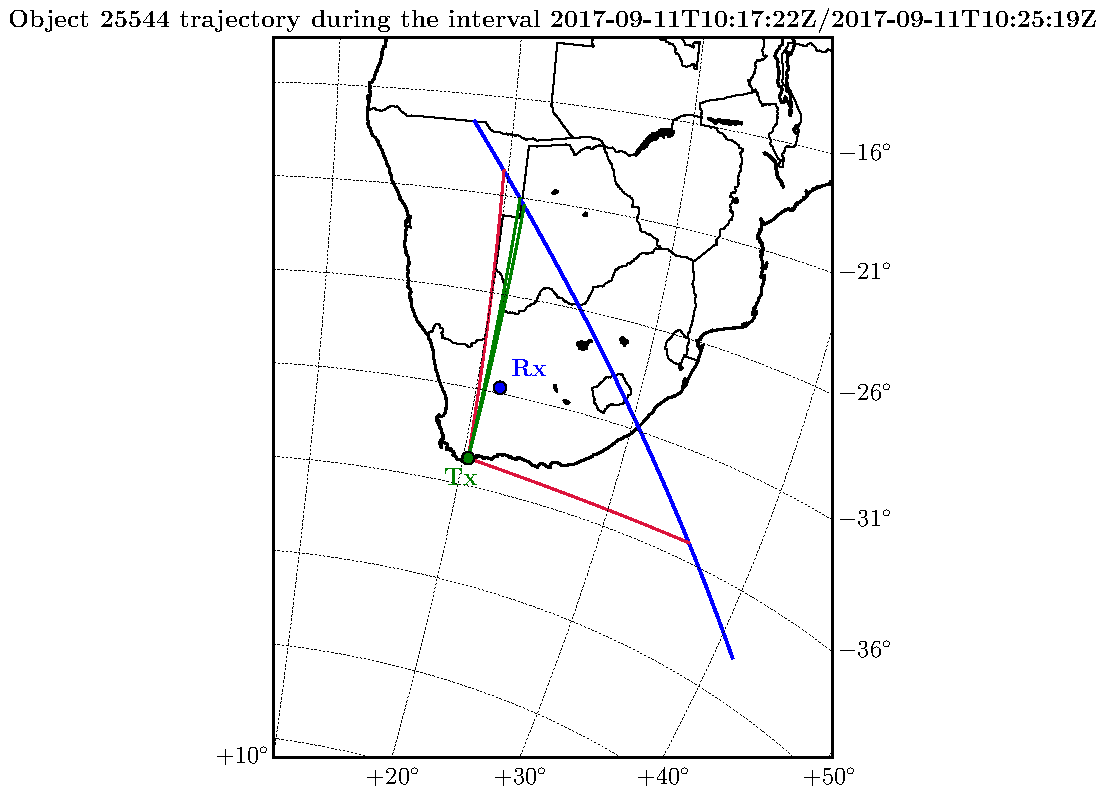
\includegraphics[scale=0.45]{main057iss14map.pdf}
	\caption{The target’s trajectory illustrated on a map (in blue). The Tx and Rx are annotated in green and blue. The region bounded by the red lines and the blue curve is the transmitter’s FoR whereas the FoV is bounded by the green lines and the blue curve.} \label{fig:schedu:map}
\end{figure}

The radar Tx is a dish antenna with a $5~\mathrm{m}$ radius. Its half-power beamwidth has been calculated to be $\Theta_{3~\mathrm{dB},\text{Tx}}=1.272^\circ$ and its gain at the beam-centre is $G_{\text{Tx}}=40.7~\mathrm{dBi}$. MeerKAT dishes have a diameter of $13.5~\mathrm{m}$. Their beamwidth is $\Theta_{3~\mathrm{dB},\text{Rx}}=0.943^\circ$ and gain at the beam centre is $G_{\text{Rx}}=43.4~\mathrm{dBi}$. Given that both the Tx and receiver (Rx) antennas are directional, their beam centres can be pointed anywhere in the sky to ensure a good radar geometry for detecting and tracking the object of interest.

The most opportune epoch for an observation experiment is when the target RSO spends a maximum amount of time, referred to as \emph{illumination time} $T_{i,Tx}$, within the Tx's beam. This ensures that the radar collects the largest possible number of data points from the target. More data points should lead to an improvement in the orbit determination accuracy of the MPT, according to the Law of Large Numbers. The chosen epoch occurs either when the target rises above the horizon or sinks below the horizon at the radar site. For the ISS case study, the best illumination time resulted from the portion of the trajectory bounded by the green lines in Figure \ref{fig:schedu:map}. The computational process for selecting a Tx antenna pointing pair $( \theta_{\text{Tx}} , \psi_{\text{Tx}})$ is explained below.

For each target position vector in the time-indexed trajectory shown in blue in Figure \ref{fig:schedu:map}, the elevation $\theta_{\text{Tx}} \lbrack k \rbrack$ and azimuth $\psi_{\text{Tx}}\lbrack k \rbrack$ angles at the radar Tx are calculated. The Tx-illumination time $T_{i,Tx}$ is found by counting how many trajectory data points $\{ \theta_{\text{Tx}}\lbrack k \rbrack,\psi_{\text{Tx}}\lbrack k \rbrack\}$ lie within a circle of radius $\Theta_{3~\mathrm{dB},\text{Tx}}=1.272^\circ$ about a test beam centre $\{ \theta_{\text{Tx}}\lbrack k_{\text{test}} \rbrack,\psi_{\text{Tx}}\lbrack k_{\text{test}} \rbrack \}$. The test beam centres are simply the elevation and azimuth angles of the target trajectory within the radar's FoR. The maximum data point count occurs at the discrete-time index of $k_{\text{max}}=848331$, which corresponds to a Tx-illumination time of $ T_{i,Tx} = 6.463280~\mathrm{s} $ and a beam centre of $\{ \theta_{\text{Tx}}\lbrack k_{\text{max}} \rbrack,\psi_{\text{Tx}}\lbrack k_{\text{max}} \rbrack \} = \{ 12.267187^\circ, 177.988607^\circ \}$. Figure \ref{fig:schedu:schedu:tx:beamcirc} shows the elevation angle versus azimuth angle plot during a portion of the target's transit through the sensor's FoR. The Tx dish antenna's beam is represented by the grey circle whose centre is at the chosen pair $\{ \theta_{\text{Tx}}\lbrack k_{\text{max}} \rbrack,\psi_{\text{Tx}}\lbrack k_{\text{max}} \rbrack \}$.

\begin{figure}[ht]
	\centering
	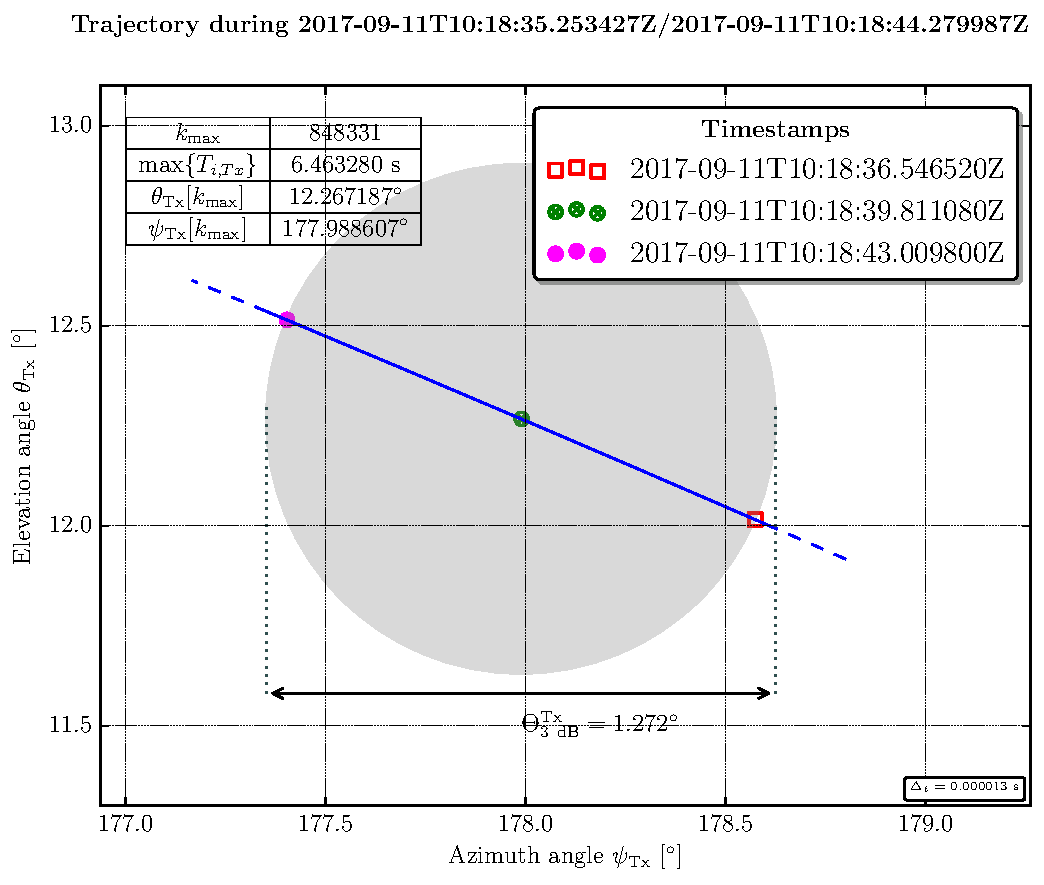
\includegraphics[scale=0.49]{main057iss08txbeamcirc0test.pdf}
	\caption[Transmitter beam centre pointing: circular beam model]{Elevation versus azimuth plot for the target's transit through the circular beam model (represented by the grey circle). The red and purple markers indicate the elevation and azimuth angle pairs at which the target entered and then left the FoV. The chosen beam centre is represented by the green marker. }
	\label{fig:schedu:schedu:tx:beamcirc}
\end{figure}

In Figure \ref{fig:schedu:schedu:tx:beamcirc}, the legend on the right indicates the estimated timestamps for the target entering the Tx's beam, crossing its beam centre and then exiting the beam. The Mission Planning Tool has thus determined how the transmitter should illuminate the target to be able to run a BPE.

The next step is to schedule the MeerKAT radar receiver. Three MeerKAT dishes are sufficient to cover the entirety of the illuminated portion of the trajectory. First, we consider the first MeerKAT dish as reference. We task \textbf{M000} as the main receiver Rx0 and aim it at the point corresponding to the target's position at maximum illumination time in the transmitter's beam. Then we task \textbf{M001} (Rx1) and \textbf{M002} (Rx2) to cover the illuminated trajectory which has not been covered by \textbf{M000}. This can be done because the MeerKAT beams can be moved independently of each other.

Figure \ref{fig:schedu:schedu:rx:10:radecnormalized} shows the target's passage on a nominal topocentric right ascension-declination (TOPORADEC) map where the main dish \textbf{M000}'s pointing is referenced as $(\Delta \alpha_t,\Delta \delta_t) = (0^\circ,0^\circ)$. The origin in the normalized TOPORADEC plot corresponds to the elevation and azimuth pair $\{\theta_{\text{Rx0}},\psi_{\text{Rx0}}\} = \{16.035918,-177.427143^\circ\}$ at the Greenwich Mean Sidereal Time angle $\theta_{\text{GMST}}=145.2960759^\circ$ (which is derived from the epoch). The elevation and azimuth angles needed to task the receive dishes are obtained from the normalized TOPORADEC plot in Figure \ref{fig:schedu:schedu:rx:10:radecnormalized}. The timestamps in the legend of Figure \ref{fig:schedu:schedu:rx:10:radecnormalized} are used to schedule the receive nodes. 

The scheduling performed by the MPT is shown in the bistatic plane in Figure \ref{fig:schedu:schedu:geom:bistaticplane}. The MeerKAT radar engineer will make use of Figure \ref{fig:schedu:schedu:geom:bistaticplane} to plan an observation experiment.

\begin{figure}[ht]
	\centering
	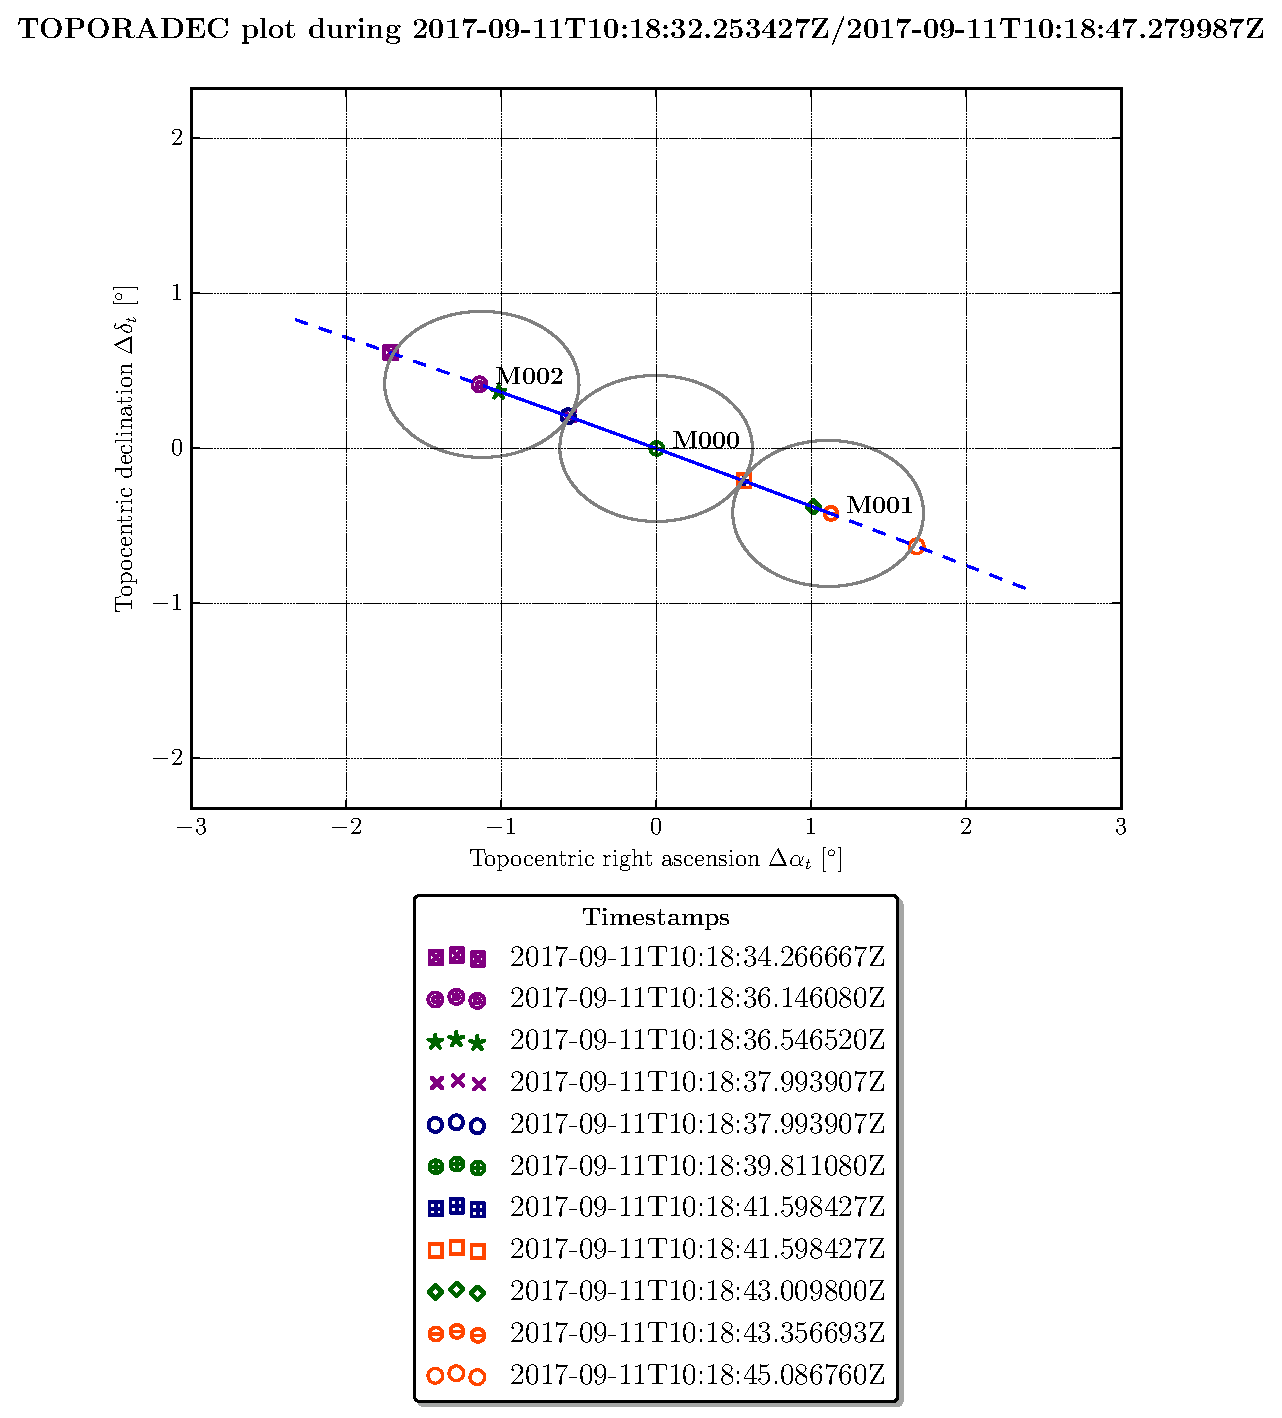
\includegraphics[scale=0.4]{main057iss100radecnormalized0test.pdf}
	\caption[Topocentric right ascension declination profile for the target's passage]{Normalized topocentric right ascension declination profile for the target's passage through the Rx's FoV. The Tx-illuminated portion of the trajectory is the solid blue curve segment. Each dish's beam (in grey) is labelled with its name. The timestamps at relevant points in the target passage are shown on the right.  }\label{fig:schedu:schedu:rx:10:radecnormalized}
\end{figure}

\begin{figure}[ht]
	\centering
	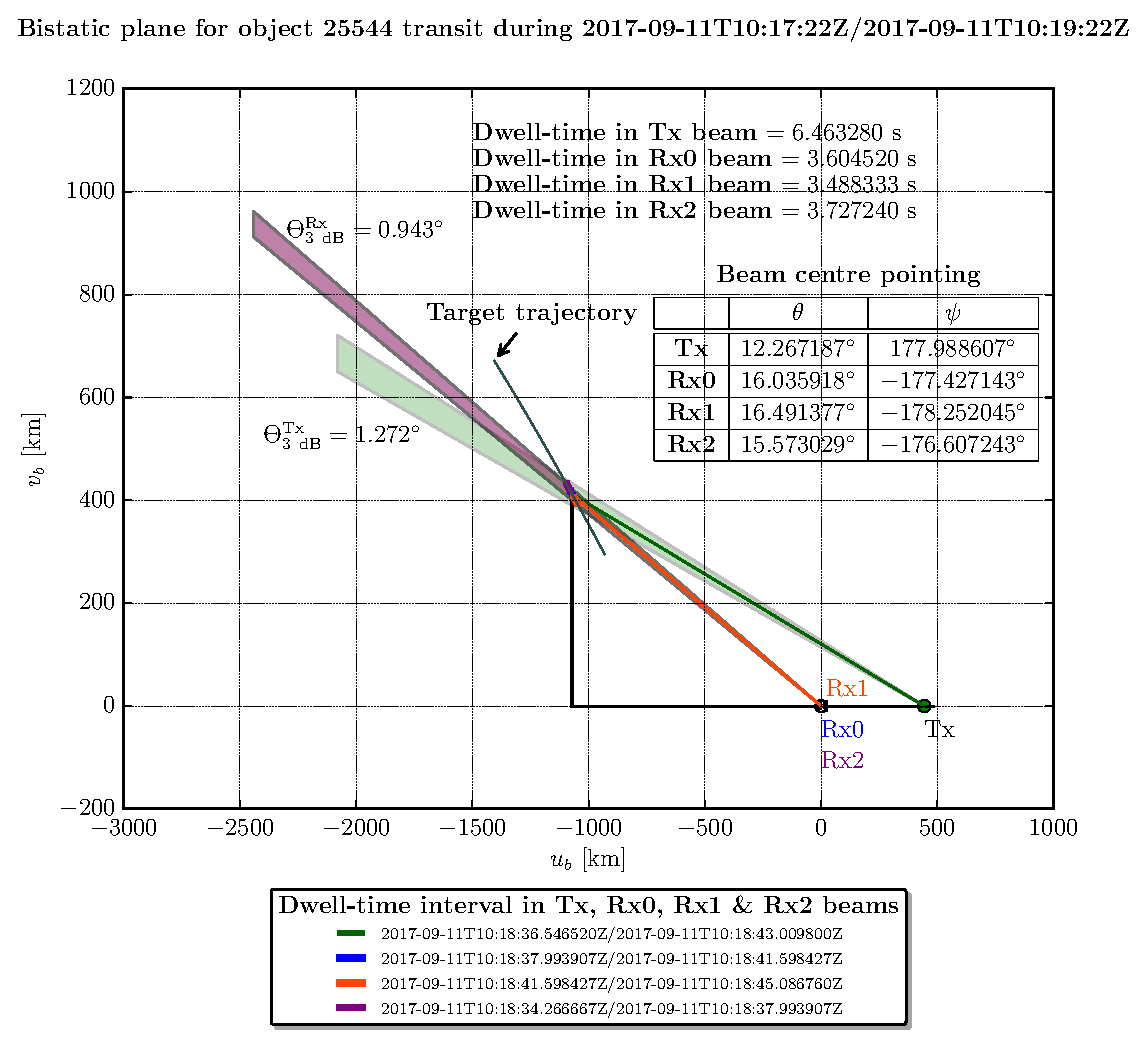
\includegraphics[scale=0.42]{main057iss111bistaticplane0.pdf}
	\caption[Target observation geometry visualized on the bistatic plane]{Target trajectory projected onto the bistatic plane. The Tx's beam is shown in green. }\label{fig:schedu:schedu:geom:bistaticplane}
\end{figure}

Space objects investigated in \cite{ashivmsc} were found to be have spent between $4.5~\mathrm{s}$ to $12.8~\mathrm{s}$ in the radar transmitter’s illuminating beam.

\subsection{Radar measurements prediction} \label{subsection:rad}
The MPT helps in quantifying the MeerKAT radar's performance in terms of its characteristics and in terms of the observation geometry and nature of the target. For the ISS observation scenario discussed previously, the single pulse power $P_\text{Rx}$ measured at the receiver was calculated with the radar equation.
\begin{equation}
P_\text{Rx} = \frac{P_\text{Tx}G_\text{Tx}G_\text{Rx}\lambda_c^2 \sigma_b}{(4\pi)^3\rho_\text{Tx}^2 \rho_\text{Rx}^2}
\label{eqn:schedu:snr:calc:singlepulse}
\end{equation}
where $P_\text{Tx}$ is the transmitted power; $G_\text{Tx}$ and $G_\text{Rx}$ are the Tx and Rx antenna gains; $\lambda_c$ is the carrier's wavelength; $\sigma_b$ is the bistatic radar cross section of the RSO; and $\rho_\text{Tx}$ and $\rho_\text{Rx}$ are the slant-ranges from the target to the Tx and Rx respectively. The Rx gain in Eqn.~\ref{eqn:schedu:snr:calc:singlepulse} is updated with the beamshape loss according to \cite[Eqn.~6]{morselli2015orbit}. For the ISS experiment, the radar cross section was taken to be $401.801~\mathrm{m}^2$. Aspect variations due to the space object of interest tumbling about its centre of mass were not accounted for in this preliminary version of the MPT. From the single pulse SNR, the coherently integrated SNR is calculated by assuming a coherent processing interval of $0.1~\mathrm{s}$. The coherent integration gain is thus $38.751~\mathrm{dB}$. The coherently integrated SNR ranges from $62.771~\mathrm{dB}$ to $65.861~\mathrm{dB}$.

The bistatic range resolution is calculated using \cite[Eqn.~11.44]{cherniakov2008bistatic}. It is then used to calculate the bistatic range measurement error \cite{curry2005radar}. The maximum range measurement error of $\sigma_{\rho \text{, b}}=7.714042 \times 10^{-6}~\mathrm{km}$ is not realistic because of the overly large radar PRF value in Table \ref{table:intro1:radparam}.

\subsection{Orbit determination}
Orbit determination is performed by the MPT based on measurements of bistatic range, elevation and azimuth angle to the target from the radar receiver. However, the current design of the MeerKAT radar does not feature an angle of arrival estimation scheme. Researchers at the Italian BIRALES radar which operates in a similar way to the MeerKAT radar developed a so-called `Observables Estimation' process to determine the elevation-azimuth angle profile of a target pass \cite{surrey814139}. It hinges on the fact that, for the RSO tracking problem, the nominal trajectory for the space object of interest is known fairly accurately. Given the nominal trajectory for a proposed observation experiment, it is possible to make the SNR calculations given in Subsection \ref{subsection:rad}.

\begin{table*}[t]
	\caption[BIRAZEL-based ISS tracking with an initial perturbation vector]{Tracking the ISS based on BIRAZEL measurements with a small initial perturbation vector $\mathbf{\delta}\mathbf{x}$.} \label{table:od2:birazel:small}
	\centering
	
		\begin{tabular}{c | r | r | r | r | r |r}
			\hline 
			Position & Actual value $[\mathrm{km}]$ & Nominal value $[\mathrm{km}]$ & Perturbation $[\mathrm{km}]$ & Estimate $[\mathrm{km}]$ & Variance $[\mathrm{km}^2]$ & Error $[\mathrm{km}]$ \\
			\hline \hline
					$x$ & $-6147.396792$ & $-6147.397083$ & $0.000290$ & $-6147.396995$ & $0.0001917650603003$ & $0.000202$ \\
			$y$ &  $1516.715741$ &  $1516.716163$ &$-0.000422$ &  $1516.715455$ & $0.0003269335854790$ & $0.000286$ \\
			$z$ & $-2435.993380$ & $-2435.993118$ & $-0.000262$ & $-2435.993447$ & $0.0002653123666930 $ & $0.000067$ \\
			\hline
			Velocity & Actual value $[\mathrm{km/s}]$ & Nominal value $[\mathrm{km/s}]$ & Perturbation $[\mathrm{km/s}]$ & Estimate $[\mathrm{km/s}]$ & Variance $[(\mathrm{km/s})^2]$ & Error $[\mathrm{km/s}]$ \\
			\hline \hline
			$\dot{x}$ & $0.774498$ & $0.774458$ & $0.000041$ & $0.774505$ & $0.0000001025960444$ & $0.000007$ \\
			$\dot{y}$ & $-5.439955$ & $-5.439988$ & $0.000033$ & $-5.439953$ & $0.0000001727778030$ & $0.000002$ \\
			$\dot{z}$ & $-5.346346$ & $-5.346331$ & $-0.000014$ & $-5.346332$ & $0.0000001707422180$ & $0.000014$\\
			\hline
		\end{tabular}%
	
\end{table*}

There is no explicit equation for the target passage in Figure \ref{fig:schedu:schedu:rx:10:radecnormalized}. The BIRALES researchers assumed that it is possible to approximate the trajectory with two parametric second-degree polynomials, one for the topocentric right ascension and one for the topocentric declination, as given in the following equations.
\begin{align}
\Delta \hat{\alpha}_t(t) &=  a_2 t^2 + a_1 t + a_0\\
\Delta \hat{\delta_t}(t) &=  b_2 t^2 + b_1 t + b_0
\label{eqn:od2:observest:toporadec}
\end{align}
where $t$ is a continuous-time variable, $\Delta \hat{\alpha}_t(t)$ and $\Delta \hat{\delta_t}(t)$ are the estimated normalized topocentric right ascension and declination. Given that the antenna pointing for \textbf{M000}, \textbf{M001} and \textbf{M002} is known accurately (determined in Subsection \ref{subsection:schedu}) and that the highest SNR is obtained when the target transits closest to the antenna beam centre, three pairs of measurements of the object's TOPORADEC profile can be made during a pass. A weighted curve fit is done (using the relative highest SNR measured by each MeerKAT receiver as weight) to obtain the value of coefficients $\{a_2,a_1,a_0\}$ and $\{b_2,b_1,b_0\}$. Figure \ref{fig:od2:observest:polynomerror:2} shows the error between the true TOPORADEC profile and the parametric second-order polynomials estimated with the weighted curve fit.

\begin{figure}[ht]
	\centering
	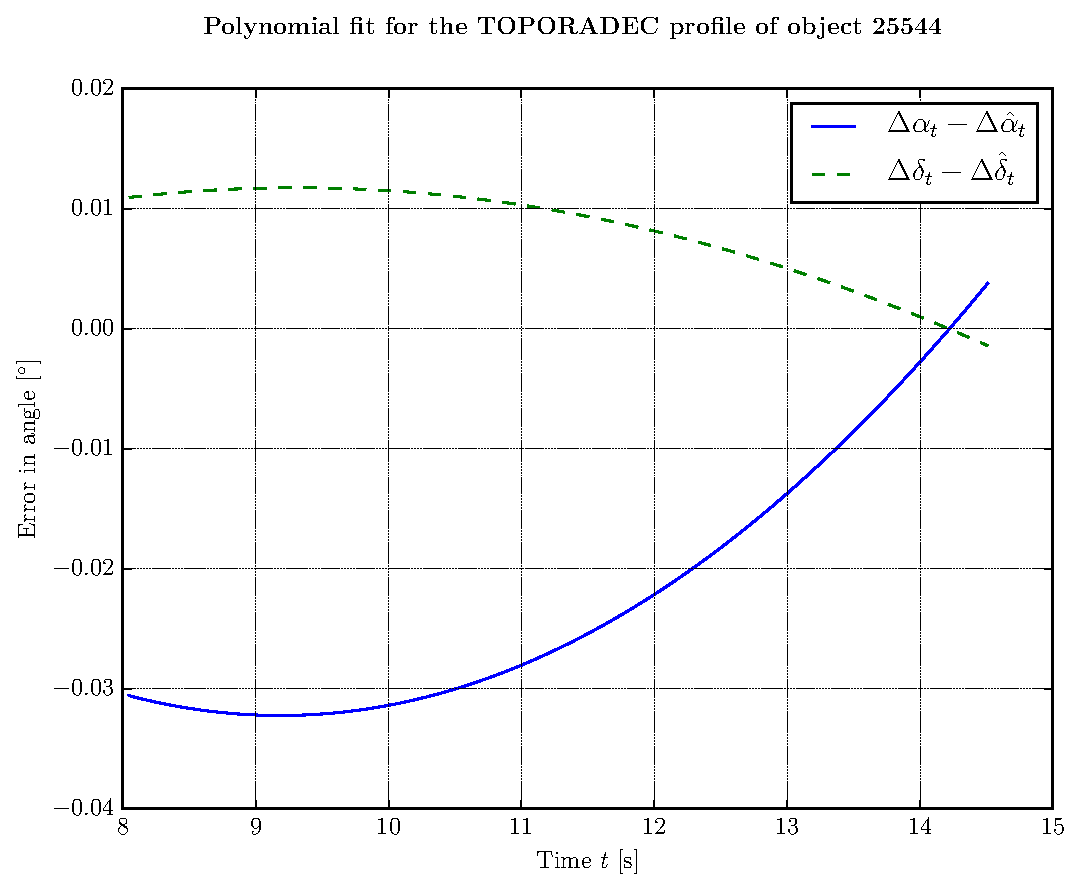
\includegraphics[scale=0.39]{main057iss41polynomerror01.pdf}
	\caption[Estimation errors in polynomial fit for the right ascension/declination profile]{Discrepancy between the true TOPORADEC profile and the estimated parametric second-order polynomials}
	\label{fig:od2:observest:polynomerror:2}
\end{figure}
Figure \ref{fig:od2:observest:polynomerror:2} shows that the estimation error for the topocentric right ascension and declination lies well within the range $-0.04^\circ$ to $0.04^\circ$. The BIRALES paper \cite{surrey814139} does not show how to account for the estimation errors in the pseudo-measurements of elevation and azimuth angle fed to the Orbit Determination processor. For simplicity, it is assumed in the radar measurement covariance matrix $\mathbf{R}$ that the standard deviations of the angle measurements are $0.04^\circ$ which is very pessimistic.

The tracking filter used to estimate the RSO's orbit was an expanding-memory Case 4\footnote{Nonlinear target dynamics, nonlinear measurement model. \cite{trackingfilterengineering}} Gauss-Newton filter \cite{trackingfilterengineering}. The target dynamic model was a two body plus $J_2$ differential equation model \cite{tapley2004}. The ground truth trajectory and the filtered trajectories were obtained by numerical integration of the target dynamic model with a fourth-order Runge-Kutta method. The target state vector $\mathbf{x}$ contained the RSO's position and velocity vectors in three dimensions in an Earth-Centered Inertial (ECI) frame. 
\begin{equation}
\mathbf{x} = \begin{bmatrix}
x & y & z & \dot{x} & \dot{y} & \dot{z}
\end{bmatrix}^T
\end{equation}
The measurement vector $\mathbf{y}$ consisted of bistatic range $\rho_\text{b}$, elevation angle $\theta_{\text{Rx}}$ and azimuth angle $\psi_{\text{Rx}}$ to the MeerKAT receiver.
\begin{equation}
\mathbf{y} = \begin{bmatrix}
\rho_\text{b} & \theta_{\text{Rx}} & \psi_{\text{Rx}}
\end{bmatrix}^T
\end{equation}
The noisy radar measurements $ \mathbf{y}_{\text{meas}}$ were simulated as the measurement vector $\mathbf{y}$ with additive measurement noise $\mathbf{\nu}$ which is normally-distributed with mean zero and covariance $\mathbf{R}$.
\begin{equation}
\mathbf{y}_{\text{meas}}= \mathbf{y} + \mathbf{\nu}
\end{equation}

To evaluate the tracking performance for the ISS observation experiment, a thousand Monte Carlo simulations were done. The initial state vector fed into the tracking filter, that is, the nominal trajectory $\mathbf{x}^\ast$ to be refined by the tracking filter, is obtained by subtracting a perturbation vector $\delta \mathbf{x}$ from the true initial trajectory $\mathbf{x}$ \cite{trackingfilterengineering}.
\begin{equation}
    \mathbf{x}^\ast = \mathbf{x} - \delta \mathbf{x}
\end{equation}
Tracking results are shown in Table \ref{table:od2:birazel:small}. All displacement and velocity values are given to six decimal places (that is, to $\mathrm{mm}$ or to $\mathrm{mm/s}$, except for variance where they are given to sixteen decimal places. The true state vector $\mathbf{x}$ for the ground truth trajectory remained unchanged in all Monte Carlo runs and is shown in the `Actual value' column in Table \ref{table:od2:birazel:small}. The `Nominal value' column contains the elements of the nominal trajectory $\mathbf{x}^\ast$; the `Perturbation' column contains the elements of the perturbation vector $\delta \mathbf{x}$; the entries in the `Estimate' column are the elements of the average estimated state vector $\hat{\mathbf{x}}$; ; the `Variance' column contains the diagonal elements of the filter covariance matrix averaged over a thousand Monte Carlo runs and; finally, the `Error' column contains the sample mean values of the estimate error vector $\tilde{\mathbf{x}} = \mathbf{x} - \hat{\mathbf{x}}$.



%Based on noisy measurements $\mathbf{y}_{\text{meas}}$, the measurement covariance matrix $\mathbf{R}$ and the nominal trajectory $\tilde{\mathbf{x}}$, the Gauss-Newton filter produced estimated state vectors $\hat{\mathbf{x}}$ with their corresponding covariance matrices $\hat{\mathbf{P}}$. 

%The average estimated state vector $\mathbb{E}\{\mathbf{x}\}$ over $1000$ Monte Carlo runs is shown in the `Estimate' column of Table \ref{table:od2:birazel:small}. The corresponding elements from the average estimated covariance matrix are shown in the `Variance' column of Table \ref{table:od2:birazel:small}. The error  $\mathbb{E}\{\tilde{\mathbf{x}}\}$ between the average state vector estimate $\hat{\mathbf{x}}$ and the true state vector $\mathbf{x}$ is shown in the `Error' column of Table \ref{table:od2:birazel:small}. The estimation errors are found to be of comparable magnitude to the perturbation vector $\mathbf{\delta} \mathbf{x}$ in the initial nominal trajectory, with an estimated position error of less than $1~\mathrm{m}$. 
%Two more sets of Monte Carlo experiments were done with initial perturbation vectors which were 10 and 100 times larger ($10\mathbf{\delta} \mathbf{x}$ and $100\mathbf{\delta} \mathbf{x}$) and it was found that the estimation errors were then much smaller in comparison to the perturbation in the initial nominal trajectory. These results are not shown here for the sake of brevity but the estimated position error was less than $1~\mathrm{m}$ in both cases. These numerical results show that the orbit of a RSO can be accurately estimated from a single target pass through the MeerKAT radar's FoV even when the preliminary orbit is inaccurately known.

%This subsection has shown how an observed space object's orbit can be estimated from measurements made by the MeerKAT radar.

The estimation errors in Table \ref{table:od2:birazel:small} are smaller than the perturbation vector added to the initial trajectory, indicating that the tracking filter is improving the accuracy of the orbit track.

\section{Conclusions} \label{section:conclusions}
%The Mission Planning Tool described in this paper predicts the achievable performance of the proposed South African MeerKAT radar meant for space object detection, tracking and imaging. A feasibility study of this proposed bistatic radar system is being done in the Radar Remote Sensing Group at the University of Cape Town in South Africa. This paper discusses the operation of the MPT by investigating an International Space Station observation scenario. Numerical simulations are done by the MPT to assist in scheduling the bistatic radar to perform an observation experiment, to calculate the predicted radar measurements and errors as well as to estimate the orbit of the observed object. 

The proposed MeerKAT radar system will be a first step towards developing a Space Situational Awareness capacity in South Africa. The tailor-made MeerKAT radar Mission Planning Tools described in this paper predicts the achievable performance of the MeerKAT radar with respect to its intended purpose of detecting and tracking space objects. To illustrate the functionality of the MeerKAT radar MPT, this paper explores an International Space Station observation scenario. 

The results show that, with the help of the Mission Planning Tool, the proposed MeerKAT radar can be feasibly scheduled to observe and track space objects in the LEO regime based on a single target pass. The tailor-made orbit determination phase of the MPT enables statistical orbit determination with a single target pass through the MeerKAT radar's Field of View to a good degree of accuracy (estimated errors of less than $1~\mathrm{m}$ in position and less than $1~\mathrm{mm/s}$ in velocity). 

The final MeerKAT radar system design will make use of a different, more realistic, pulse repetition frequency than the one stated in Table \ref{table:intro1:radparam}. Due to this change in PRF, the simulations done with the MPT will have to be re-run to determine the actual performance of the proposed MeerKAT radar. It is also recommended, in future work, to investigate aperture beamforming to exploit the large number of MeerKAT dishes available. This will result in high resolution images with reduced angular measurement errors. These, in turn, will contribute to more accurate orbits being estimated by the OD phase of the MPT.

The MeerKAT array is a precursor to the Square Kilometre Array which will become fully operational in 2030. The SKA will be the largest radio telescope in the world thanks to its physically distant cores - one will be in South Africa and the other will be in Australia. Very Long Baseline Interferometry 
(VLBI)  can be used to create high resolution images of large portions of the sky to survey a vast amount of space debris as well as track space objects. VLBI at the SKA for tracking
debris is a possibility if powerful radar transmitters are
% \newpage 
%% to balance the end.
available to illuminate space targets. VLBI-based space object observations with the SKA can be investigated in future work closer to 2030.


\addtolength{\textheight}{-15cm}   % This command serves to balance the column lengths
                                  % on the last page of the document manually. It shortens
                                  % the textheight of the last page by a suitable amount.
                                  % This command does not take effect until the next page
                                  % so it should come on the page before the last. Make
                                  % sure that you do not shorten the textheight too much.

%%%%%%%%%%%%%%%%%%%%%%%%%%%%%%%%%%%%%%%%%%%%%%%%%%%%%%%%%%%%%%%%%%%%%%%%%%%%%%%%



%%%%%%%%%%%%%%%%%%%%%%%%%%%%%%%%%%%%%%%%%%%%%%%%%%%%%%%%%%%%%%%%%%%%%%%%%%%%%%%%



%%%%%%%%%%%%%%%%%%%%%%%%%%%%%%%%%%%%%%%%%%%%%%%%%%%%%%%%%%%%%%%%%%%%%%%%%%%%%%%%
\section*{ACKNOWLEDGMENT}

This research was supported by a block grant accorded to Professor Inggs by the South African Radio Astronomy Observatory.



%%%%%%%%%%%%%%%%%%%%%%%%%%%%%%%%%%%%%%%%%%%%%%%%%%%%%%%%%%%%%%%%%%%%%%%%%%%%%%%%

\begin{thebibliography}{99}
\bibitem{odpo}
{NASA Orbital Debris Program Office}, ``Frequently-asked questions.''
https://www.orbitaldebris.jsc.nasa.gov/faq.html.
\newblock [Accessed 24 November 2017].

\bibitem{mehrholz2002detecting}
D.~Mehrholz, L.~Leushacke, W.~Flury, R.~Jehn, H.~Klinkrad, and M.~Landgraf,
``Detecting, tracking and imaging space debris,'' {\em {ESA Bulletin(0376-4265)}}, no.~109, pp.~128--134, 2002.

\bibitem{spsiaw}
M.~Rathnasabapathy, C.~Nwosa, and et~al., ``{Space Situational Awareness},''
tech. rep., {Space Generation Advisory Council}, 2012.
\newblock {Space Situational Awareness Educational Series}.

\bibitem{esaklinkrad}
H.~Klinkrad, T.~Donath, and T.~Schildknecht, ``Investigations of the
feasibility of a european space surveillance system.'' Online. [Accessed May
1st, 2016].
		
\bibitem{krag2010european}
H.~Krag, H.~Klinkrad, T.~Flohrer, E.~Fletcher, and N.~Bobrinsky, ``{The
European space surveillance system required performance and design concepts},'' in {\em Proceedings}, 2010.

\bibitem{doreenphd}
Doreen Agaba.
\newblock {\em {Radar System Design for Detection, Tracking and Classification
  of Space Debris}}.
\newblock PhD thesis, {University of Cape Town}, 2018.

\bibitem{ashivmsc}
Ashiv~Rao Dhondea.
\newblock {Mission Planning Tool for space debris studies with the MeerKAT
  radar}.
\newblock Master's thesis, {University of Cape Town}, Cape Town, South Africa,
  2018.

\bibitem{doreenreport}
		D.~Agaba, ``{MeerKAT radar parameters},'' tech. rep., University of Cape Town,
		Department of Electrical Engineering, November 2016.

\bibitem{pysgp4}
B.~Rhodes, ``python-sgp4 package.'' https://pypi.python.org/pypi/sgp4/
\newblock [Accessed 15 March 2017].
		
\bibitem{morselli2015orbit}
A.~Morselli, R.~Armellin, P.~Di~Lizia, F.~B. Zazzera, E.~Salerno, G.~Bianchi,
S.~Montebugnoli, A.~Magro, and K.~Z. Adami, ``Orbit determination of space debris using a bi-static radar configuration with a multiple-beam receiver,''in {\em Proceedings of the 65th International Astronautical Congress 2014(IAC 2014)}, vol.~3, pp.~1774--1784, 2015.
		
\bibitem{cherniakov2008bistatic}
M.~Cherniakov, {\em Bistatic radars: Emerging technology}.
\newblock John Wiley \& Sons, 2008.
		
		\bibitem{curry2005radar}
		G.~Curry, {\em Radar System Performance Modeling}.
		\newblock Artech House radar library, Artech House, 1~ed., 2005.
		
		\bibitem{surrey814139}
		P.~D. Lizia, M.~Massari, M.~Losacco, G.~Bianchi, A.~Mattana, G.~Pupillo,
		C.~Bortolotti, M.~Roma, A.~Morselli, R.~Armellin, G.~Pupillo, A.~Magro,
		D.~Cutajar, C.~Portelli, and M.~Reali, ``Performance assessment of the
		multibeam radar sensor birales for space surveillance and tracking,'' in {\em
			7th European Conference on Space Debris}, 2017.
		
		\bibitem{trackingfilterengineering}
		N.~Morrison, {\em {Tracking Filter Engineering: The Gauss Newton and Polynomial
				Filters}}.
		\newblock {Radar, Sonar and Navigation Series 23}, {Institution of Engineering
			and Technology}, 2013.
		

	\bibitem{tapley2004}
		B.~Tapley, B.~Schutz, G.~Born, {\em {Statistical Orbit Determination}}.
		\newblock {Elsevier Academic Press}, 2004.





\end{thebibliography}




\end{document}
